\documentclass[11pt]{article}
\input{/Users/markwang/.preamble}
\begin{document}




\textbf{Part 1: DCGAN}

\begin{enumerate}
    \item \textbf{Padding} Given input dimension $W$, kernal size $K=4$, stride $S=2$, to downsample the input volume by a factor of 2, the desired output dimension is $\rfrac{1}{2} W$. We calculate the proper padding $P$ with given formula
    \[
        \frac{1}{2} W = (W - F + 2P) / S + 1 = \frac{1}{2}W - 2 + P + 1
        \qquad \Rightarrow \qquad 
        P = 1
    \]
    \item \textbf{DCGAN experiment}
    Below output image from iteration 200 and iteration 4000
    \begin{center}
        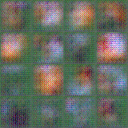
\includegraphics[width=6cm]{../samples_vanilla/sample-000200.png}
        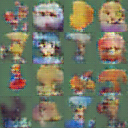
\includegraphics[width=6cm]{../samples_vanilla/sample-004000.png}
    \end{center}
    The quality of generated images do improve. In particular, the output image at iteration 200 is blurry, while the output image at iteration looks sharper and contains more details. Additionally, the colors of the images at latter iterations are generally uniform, and are devoid of color noises.
\end{enumerate}

\newpage

\textbf{Part 2: CycleGAN Experiment}
\begin{enumerate}
    \item CycleGan without cycle-consistency loss. Below are samples from generator $G_{X\rightarrow Y}$ and $G_{Y\rightarrow X}$ at iteration 600 
    \begin{center}
        
\includegraphics[width=6cm]{../samples_cyclegan/sample-000600-X-Y.png}
        
\includegraphics[width=6cm]{../samples_cyclegan/sample-000600-Y-X.png}
    \end{center}
    \item CycleGan with cycle-consistency loss. Below are samples from generator $G_{X\rightarrow Y}$ and $G_{Y\rightarrow X}$ at iteration 600
    \begin{center}
        
\includegraphics[width=6cm]{../samples_cyclegan_cycle/sample-000600-X-Y.png}
        
\includegraphics[width=6cm]{../samples_cyclegan_cycle/sample-000600-Y-X.png}
    \end{center}
    \item Pretrained CycleGan without cycle-consistency loss. Below are samples from generator $G_{X\rightarrow Y}$ and $G_{Y\rightarrow X}$ at iteration 100
    \begin{center}
        
\includegraphics[width=6cm]{../samples_cyclegan_pretrained/sample-000100-X-Y.png}
        
\includegraphics[width=6cm]{../samples_cyclegan_pretrained/sample-000100-Y-X.png}
    \end{center}
    \item Pretrained CycleGan with cycle-consistency loss. Below are samples from generator $G_{X\rightarrow Y}$ and $G_{Y\rightarrow X}$ at iteration 100
    \begin{center}
        
\includegraphics[width=6cm]{../samples_cyclegan_cycle_pretrained/sample-000100-X-Y.png}
        
\includegraphics[width=6cm]{../samples_cyclegan_cycle_pretrained/sample-000100-Y-X.png}
    \end{center}
    \item There are obvious color shift and small shape deformaties in result of models without cycle consistency. Models with cycle consistency are relatively more capable of preserving the color and structure of the input image better. This is because cycle consistency loss constrains the generators such that the intermediate image $G_{X\rightarrow Y}(x)$ preserves enough structure/information to make reconstruction as close to input image as possible, i.e. $G_{Y\rightarrow X}(G_{X\rightarrow Y}(x)) \sim x$. One positive observation is that the generator is able to capture some important characteristic of data, i.e. $X$ and $Y$. For example, $G_{X\rightarrow Y}$ is able to add black frames to images in $X$, a characteristic of images in domain $Y$, and vice versa. The reason that this happens maybe as follows. The discriminator at some point pick up that the presence and absence of black frames is an important feature in the classification process. With the goal of minimizing the loss, the generator at some later point learns the exact same feature. The fact that the generator is able to capture structure of data in an unsupervised manner is a result of this important idea behind GANs. Another observation is that training longer epochs do give a better model. The effect is similar to what we observed in DCGAN's case, where training the model for longer epochs is able to make generator output images with less color noise and sharper texture. This improvement is probably a result of the model being able to pick up structure of the data, i.e. a sharp edge in the input image probably correspond to a sharp edge in the output image, or a uniform patch of color in the input probably corresponds to a uniform patch of color in the output.
\end{enumerate}
 

  
 

\end{document}
